% ============================================================
%  EE 315 Assignment 13 - Stepped Distance Protection
%  Compile with pdfLaTeX (default on Overleaf).
%  >>> TEAM MEMBERS: edit ONLY the "EDIT HERE" block below. <<<
% ============================================================
\documentclass[11pt,a4paper]{article}
\usepackage[margin=2.4cm]{geometry}
\usepackage{graphicx,float,booktabs,amsmath,amssymb,array,xcolor,listings,hyperref,fancyhdr,caption}
\usepackage[T1]{fontenc}
\hypersetup{colorlinks=true,urlcolor=blue,linkcolor=black}

% ---------------- EDIT HERE ----------------
\newcommand{\MemberName}{Mayur Soni}
\newcommand{\MemberNo}{Member 4}
\newcommand{\RollNo}{240002037}
\newcommand{\GroupNo}{04}
\newcommand{\RepoURL}{https://github.com/Mayursoni08/Assignment13_PS}
\newcommand{\DemoURL}{https://mayursoni08.github.io/Assignment13_PS/}
% Group members table: Roll number & Name (one row each)
\newcommand{\GroupTable}{%
Member 1 & 240002007 & Akarsh J\\
Member 2 & 240002073 & Sreehari J.\\
Member 3 & 240002043 & Naman V Shetty\\
Member 4 & 240002037 & Mayur Soni [Project Lead]\\
Member 5 & 240002017 & Bhasuru Nikhil\\
Member 6 & 240002069 & Ridhi Shakkar\\}
% -------------------------------------------

\pagestyle{fancy}\fancyhf{}
\lhead{EE 315 Assignment 13}\rhead{\MemberName\ --- \RollNo}\cfoot{\thepage}
\setlength{\headheight}{14pt}
\lstset{language=Python,basicstyle=\ttfamily\tiny,breaklines=true,numbers=left,
        numberstyle=\tiny\color{gray},frame=single,keywordstyle=\color{blue}}
\newcolumntype{C}{>{\centering\arraybackslash}X}

\begin{document}

\begin{center}
{\LARGE\bfseries EE 315 Assignment 13}\\[6pt]
{\Large\bfseries Stepped Distance Protection of a 220\,kV Transmission Line:\\ Design and Verification using Simulation Data}\\[10pt]
\begin{tabular}{ll}
Course & EE 315 -- Power Systems\\
Assignment & Project / Assignment 13\\
Member Name & \MemberName\ (\MemberNo)\\
Roll Number & \RollNo\\
Project Lead & Mayur Soni\\
Group & \GroupNo\\
Project Files & \url{\RepoURL}\\
Web Demo & \url{\DemoURL}\\
\end{tabular}
\end{center}

\section{Group Members}
\begin{center}\begin{tabular}{lll}\toprule
Member & Roll Number & Name\\\midrule
\GroupTable
\bottomrule\end{tabular}\end{center}

\section{Introduction}
The objective of this assignment is to implement a stepped (three-zone) distance protection scheme for a power system and to verify it using simulation data. A distance relay measures the apparent impedance $Z_{app}=V/I$ at its location; since this is proportional to the distance to the fault, the relay can decide whether a fault lies inside its reach. ``Stepped'' means that several zones of increasing reach are used with increasing time delay, so that Zone~1 clears faults on the protected line instantly, while Zones~2 and~3 give time-delayed backup for the line itself and the adjacent lines.

A 220\,kV test system is modelled in Python. Three fault types (A-G, B-C and A-B-C) are applied at many locations. The relay voltages and currents are synthesised as sampled waveforms, phasors are estimated with a full-cycle DFT (Lecture~33), the apparent impedance is computed, and a mho characteristic decides the zone and the trip time. The same model is available as an interactive web page.

\section{System Modelling}
Relay R is at Bus~A and protects line AB. Lines BC and BD are the adjacent lines (Fig.~\ref{fig:sys}). A single source with short-circuit level 5000\,MVA supplies the system; no load current is modelled.
\begin{figure}[H]\centering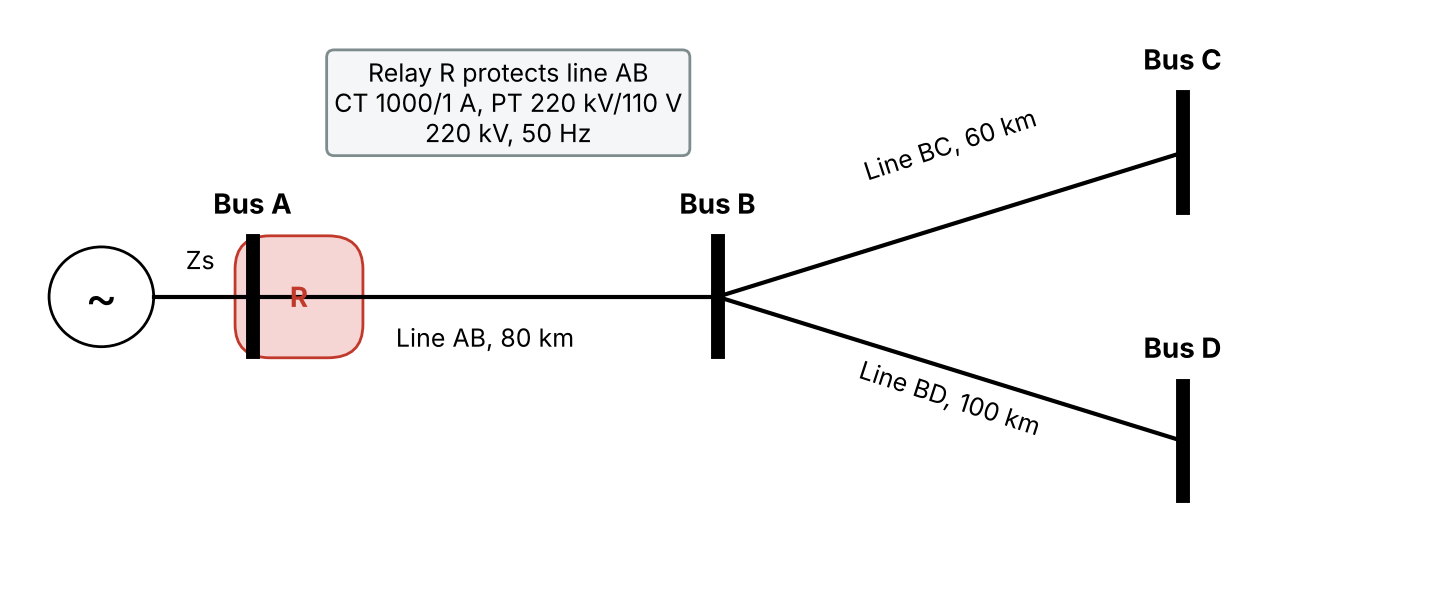
\includegraphics[width=0.85\textwidth]{figs/fig1_system.png}
\caption{Single-line diagram of the test system.}\label{fig:sys}\end{figure}

\subsection{System Parameters}
\begin{center}\small\begin{tabular}{@{}p{5.2cm}p{9cm}@{}}\toprule
Parameter & Value\\\midrule
System frequency / voltage & 50\,Hz, 220\,kV (line-line)\\
Line lengths & AB = 80\,km, BC = 60\,km, BD = 100\,km\\
Positive-sequence impedance $Z_1$ & $0.08+j0.40~\Omega$/km ($|Z_1|=0.4079$, $78.7^\circ$)\\
Zero-sequence impedance $Z_0$ & $0.30+j1.20~\Omega$/km\\
Source impedance (5000\,MVA) & $Z_{s1}=9.68\angle85^\circ~\Omega$, $Z_{s0}=12.58\angle80^\circ~\Omega$\\
CT / PT & 1000/1\,A and 220\,kV/110\,V ($Z_{sec}=0.5\,Z_{pri}$)\\
Sampling & 32 samples/cycle (1.6\,kHz)\\
Fault resistance (primary) & A-G: 5\,$\Omega$, B-C: 2\,$\Omega$, A-B-C: 1\,$\Omega$\\
Noise, harmonics & 0.1\,\% of rated peak noise, 2\,\% third harmonic, random inception angle\\
Decision window & 20--40\,ms after fault inception (2nd cycle)\\
\bottomrule\end{tabular}\end{center}

\section{Theoretical Analysis}
\subsection{Apparent impedance}
For phase faults the relay uses the line-line loop, and for ground faults the phase-ground loop with residual compensation:
\begin{align}
Z_{app}^{BC} &= \frac{V_b-V_c}{I_b-I_c}, \qquad Z_{app}^{ABC}=\frac{V_a-V_b}{I_a-I_b},\\
Z_{app}^{AG} &= \frac{V_a}{I_a+k_0\,(I_a+I_b+I_c)}, \qquad k_0=\frac{Z_{0L}-Z_{1L}}{3Z_{1L}}.
\end{align}

\subsection{Fault currents}
With the source behind the relay and a fault at distance $d$, $Z_1=Z_2=Z_{s1}+z_1 d$ and $Z_0=Z_{s0}+z_0 d$. With $E$ the source phase voltage:
\begin{align*}
\text{A-G:}&\quad I_0=I_1=I_2=\frac{E}{Z_1+Z_2+Z_0+3R_f}\\
\text{B-C:}&\quad I_1=-I_2=\frac{E}{Z_1+Z_2+R_f},\quad I_0=0\\
\text{A-B-C:}&\quad I_1=\frac{E}{Z_1+R_f},\quad I_2=I_0=0
\end{align*}
Relay voltages are $V_1=E-I_1Z_{s1}$, $V_2=-I_2Z_{s1}$, $V_0=-I_0Z_{s0}$, and phase quantities follow from the symmetrical-component transformation with $a=1\angle120^\circ$.

\subsection{Mho characteristic and zone settings}
The mho characteristic is a circle through the origin with diameter $Z_r$ along the maximum-torque angle $\theta=78.7^\circ$; the relay operates when $|Z_{app}-\tfrac{Z_r}{2}e^{j\theta}|<\tfrac{|Z_r|}{2}$. It is inherently directional. The reaches are
\[
Z_{r1}=0.8\,Z_{AB},\qquad Z_{r2}=Z_{AB}+0.5\,Z_{BC},\qquad Z_{r3}=Z_{AB}+1.2\,Z_{BD},
\]
with $Z_{AB}=32.63$, $Z_{BC}=24.48$, $Z_{BD}=40.79~\Omega$ (BC is the shortest and BD the longest adjacent line).
\begin{table}[H]\centering\small
\begin{tabular}{ccccccc}\toprule
Zone & Reach (primary) & Reach (secondary) & Reach (km) & Delay & Trip time\\\midrule
Z1 & 26.11\,$\Omega$ & 13.05\,$\Omega$ & 64  & 0\,s   & 0.04\,s\\
Z2 & 44.87\,$\Omega$ & 22.44\,$\Omega$ & 110 & 0.4\,s & 0.44\,s\\
Z3 & 81.58\,$\Omega$ & 40.79\,$\Omega$ & 200 & 1.0\,s & 1.04\,s\\\bottomrule
\end{tabular}
\caption{Zone settings. Trip time includes 40\,ms (two cycles) for data window and decision.}
\end{table}
\textbf{Coordination.} The Zone~2 delay (0.4\,s) equals the downstream Zone~1 clearing time (0.02\,s + 0.08\,s breaker + 0.3\,s margin). Zone~2 reach (44.87\,$\Omega$) stays below $Z_{AB}+0.8Z_{BC}=52.2~\Omega$, so it never overreaches the adjacent Zone~1. The Zone~3 delay (1.0\,s) exceeds the downstream Zone~2 clearing time ($0.42+0.08+0.3=0.80$\,s).

\section{Simulation and Computational Procedure}
\begin{enumerate}
\item \textbf{Fault calculation:} sequence-network phasors for each fault type, location $d$ and resistance $R_f$.
\item \textbf{Waveform synthesis:} two pre-fault cycles, then the fault with a decaying DC offset (time constant from the loop $X/R$), 2\,\% third harmonic and Gaussian noise; scaled to CT/PT secondary values.
\item \textbf{Phasor estimation:} full-cycle DFT (Lecture~33). A digital mimic filter $y[n]=x[n]+\frac{\tau}{T_s}(x[n]-x[n-1])$, $\tau=20$\,ms, is applied to both $v$ and $i$ to remove the DC offset without changing the $V/I$ ratio.
\item \textbf{Zone decision and trip time:} mho test against Z1, Z2, Z3; trip time $=40$\,ms + zone delay.
\item \textbf{Test set:} 204 faults at 5\,\% steps on AB and BC and up to 140\,\% on BD (beyond 100\,\% of BD is a hypothetical extension to test non-operation), for the three fault types.
\end{enumerate}
To reproduce: \texttt{pip install -r requirements.txt} and \texttt{python ee315\_assignment13.py}. The script writes all figures to \texttt{figs/} and the numerical results to \texttt{results\_sweep.csv} and \texttt{results\_meta.json}.

\section{Simulation Results}
\subsection{Waveforms and phasor estimation}
\begin{figure}[H]\centering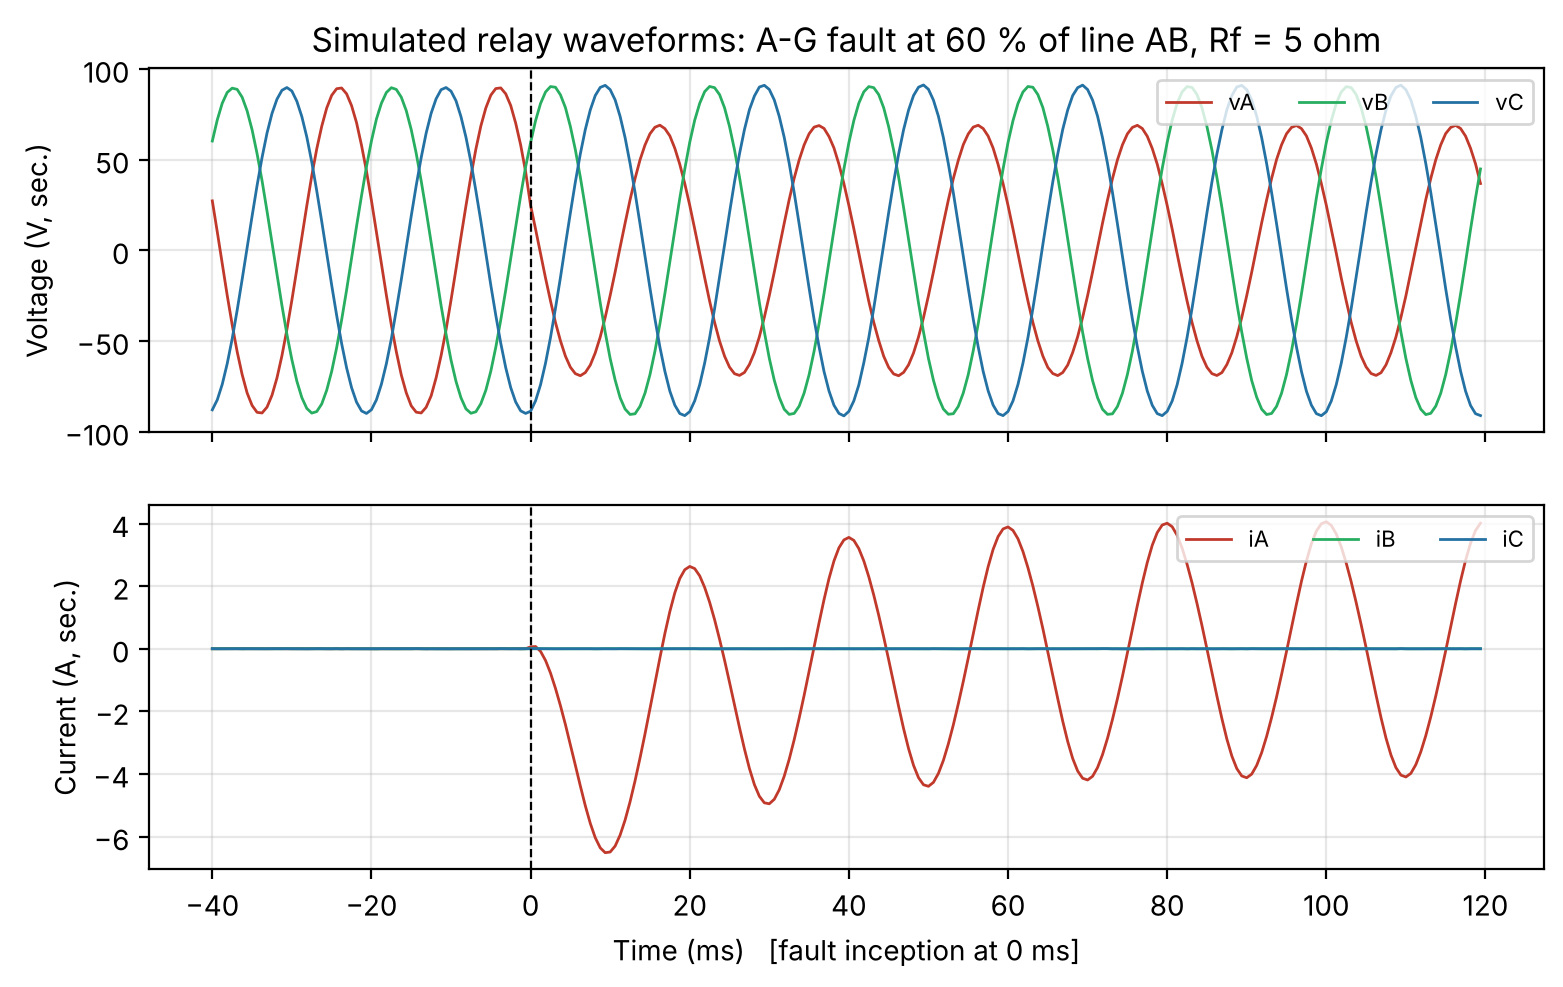
\includegraphics[width=0.68\textwidth]{figs/fig4_waveforms.png}
\caption{Simulated relay waveforms, A-G fault at 60\,\% of line AB, $R_f=5~\Omega$, at the inception angle giving maximum DC offset.}\end{figure}
\begin{figure}[H]\centering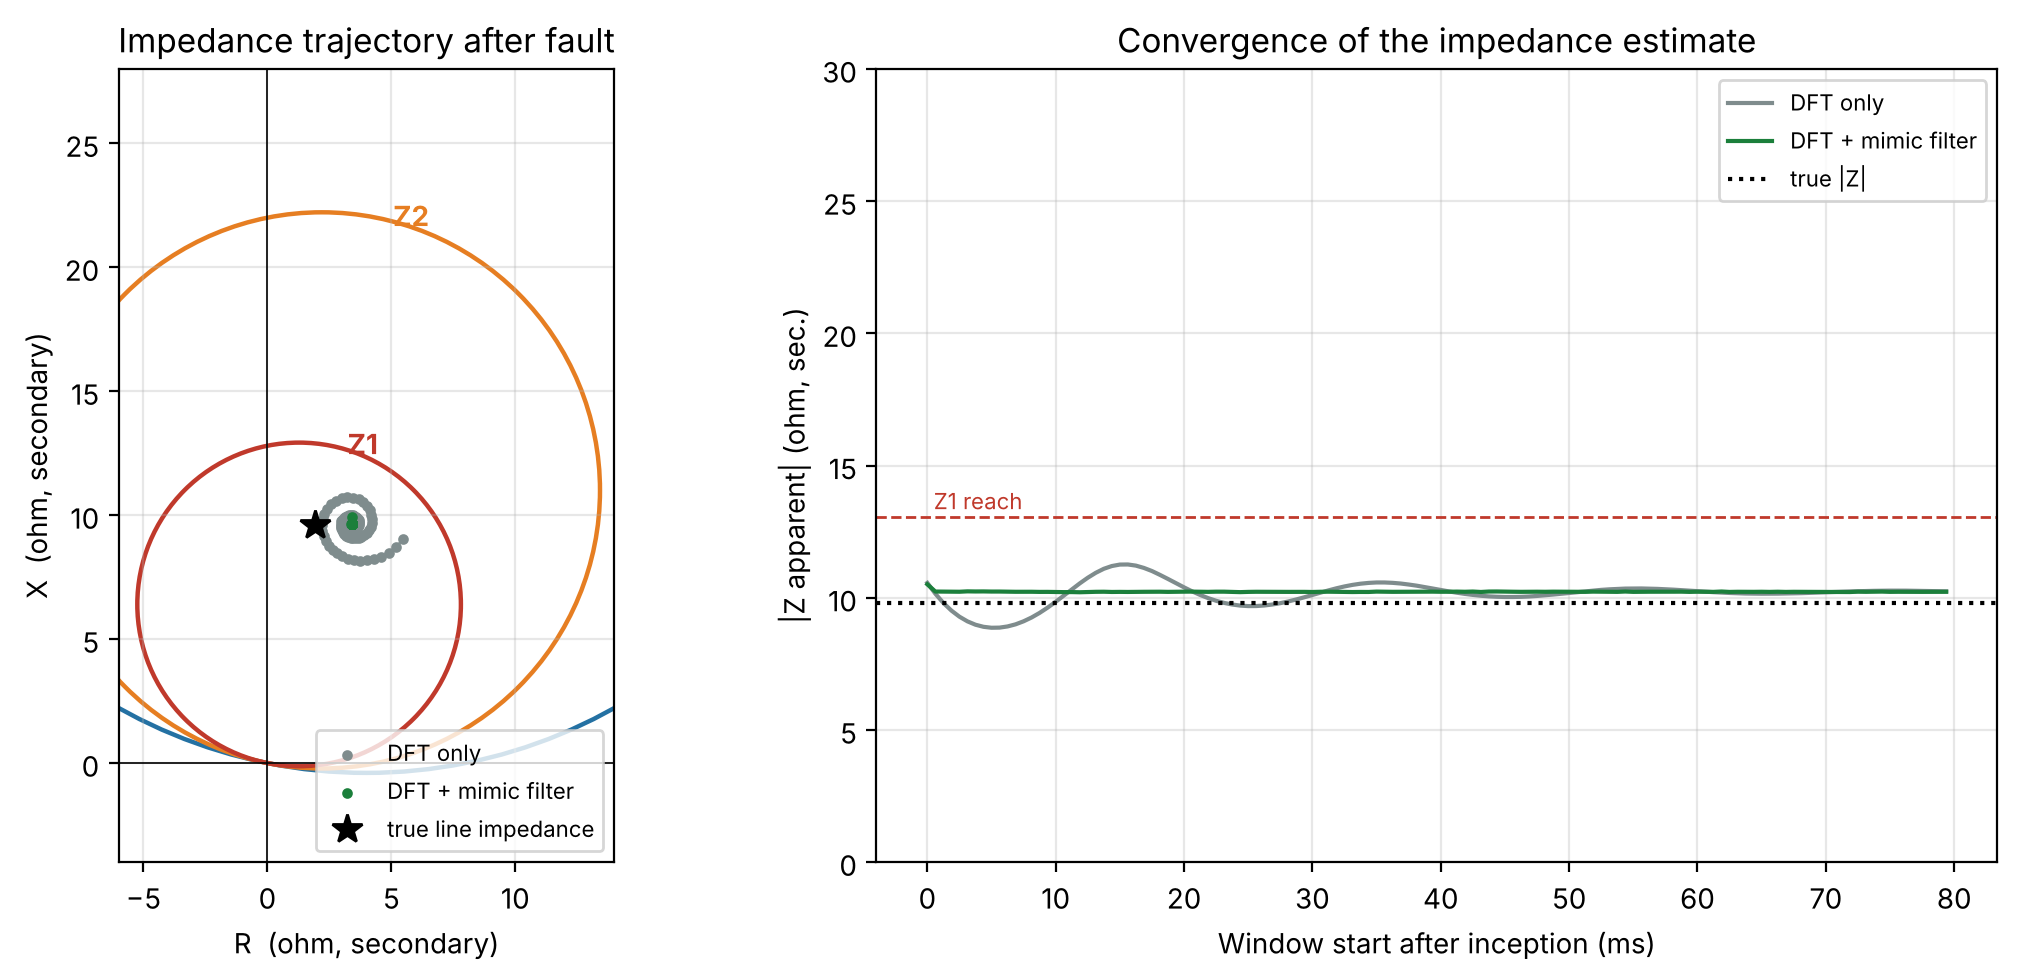
\includegraphics[width=0.9\textwidth]{figs/fig5_trajectory.png}
\caption{Apparent-impedance trajectory and magnitude after the fault, with and without the mimic filter. The offset from the true line impedance (star) is caused by $R_f=5~\Omega$; the DFT-only estimate oscillates because of the DC offset.}\end{figure}
\begin{figure}[H]\centering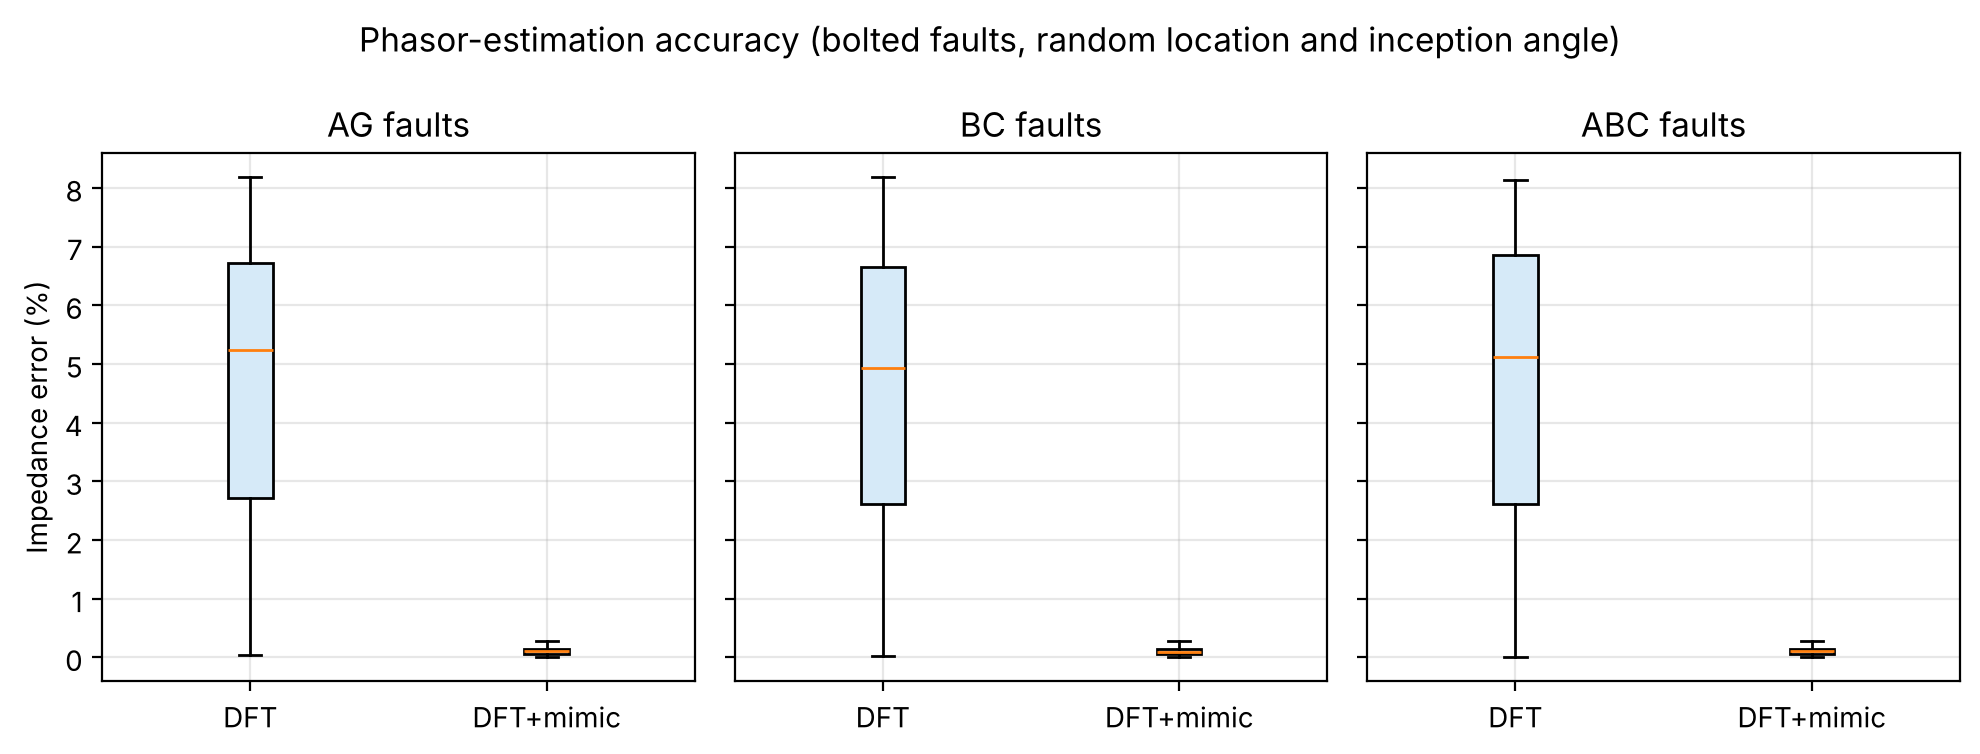
\includegraphics[width=0.7\textwidth]{figs/fig6_accuracy.png}
\caption{Impedance estimation error for 300 random bolted faults per fault type.}\end{figure}
\begin{table}[H]\centering\small
\begin{tabular}{lcc}\toprule
Fault & DFT only: mean / max error & DFT + mimic: mean / max error\\\midrule
A-G & 4.68\,\% / 8.2\,\% & 0.12\,\% / 0.78\,\%\\
B-C & 4.53\,\% / 8.2\,\% & 0.10\,\% / 0.55\,\%\\
A-B-C & 4.69\,\% / 8.1\,\% & 0.11\,\% / 0.50\,\%\\\bottomrule
\end{tabular}
\caption{Phasor-estimation accuracy.}
\end{table}

\subsection{R-X diagram}
\begin{figure}[H]\centering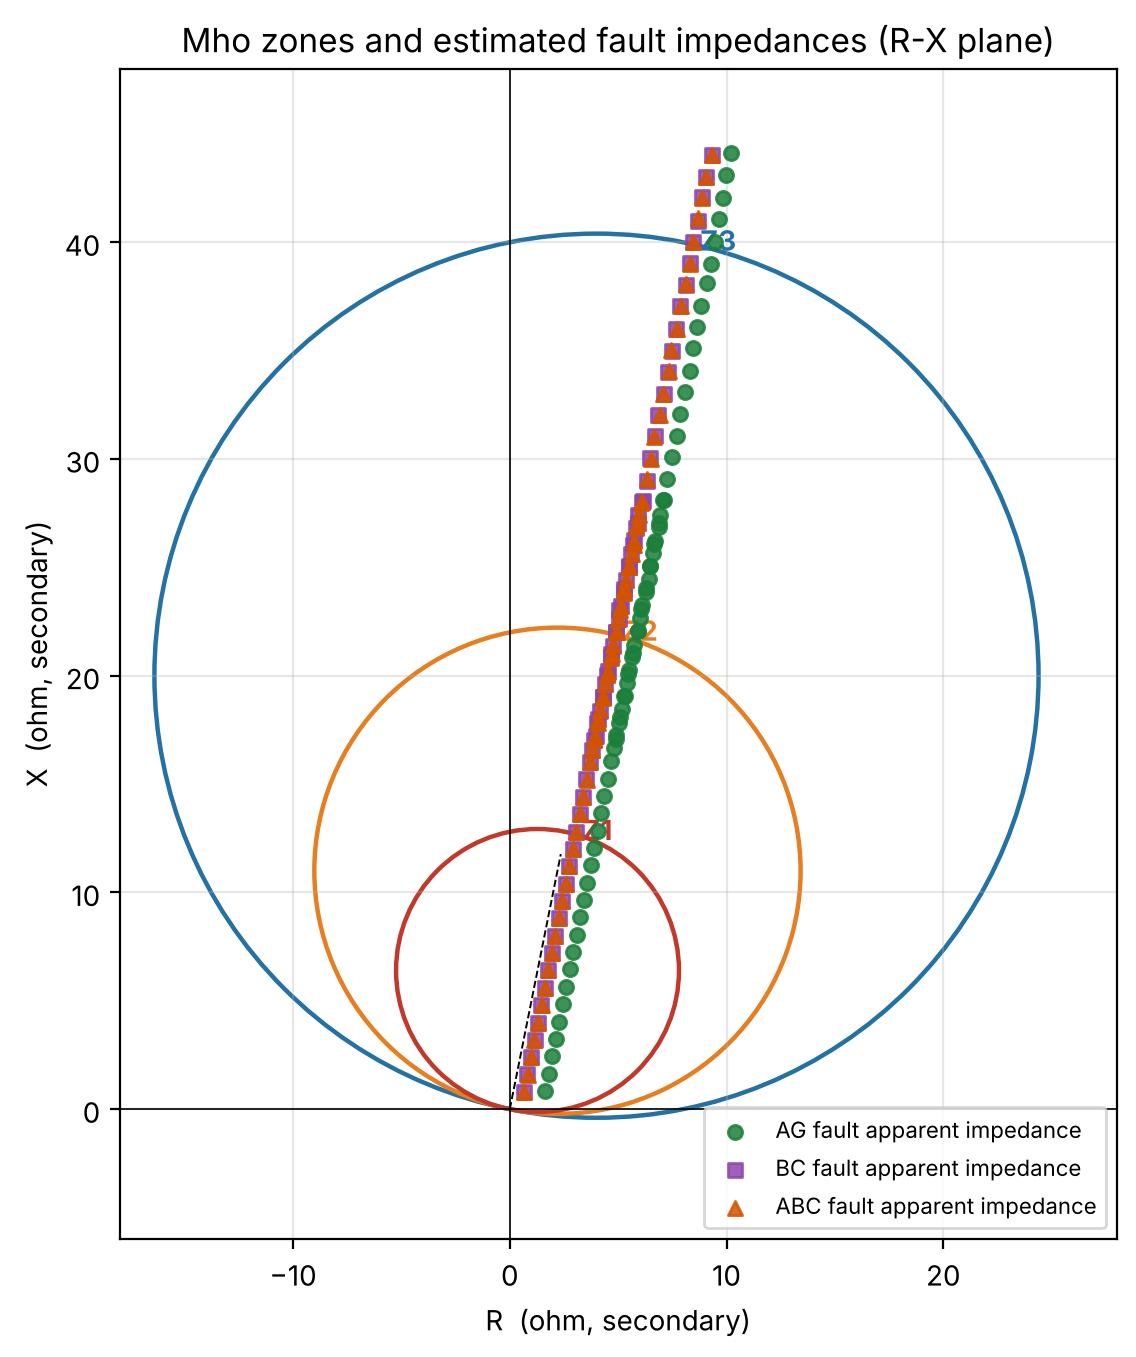
\includegraphics[width=0.58\textwidth]{figs/fig2_rx_diagram.png}
\caption{Mho zones and estimated apparent impedances of all faults on the path A-B-D.}\end{figure}

\subsection{Zone pickup and trip times}
\begin{table}[H]\centering
\footnotesize\begin{tabular}{lrccccc}\toprule
Fault location & $d$ (km) & Ideal & A-G $Z_{app}$ ($\Omega$) & A-G & B-C & A-B-C\\\midrule
Line AB, 10\% & 8 & Z1 & $1.8+1.6j$ & Z1 / 0.04 & Z1 / 0.04 & Z1 / 0.04\\
Line AB, 50\% & 40 & Z1 & $3.1+8.0j$ & Z1 / 0.04 & Z1 / 0.04 & Z1 / 0.04\\
Line AB, 70\% & 56 & Z1 & $3.7+11.3j$ & Z1 / 0.04 & Z1 / 0.04 & Z1 / 0.04\\
Line AB, 90\% & 72 & Z2 & $4.4+14.5j$ & Z2 / 0.44 & Z2 / 0.44 & Z2 / 0.44\\
Line AB, 100\% & 80 & Z2 & $4.7+16.1j$ & Z2 / 0.44 & Z2 / 0.44 & Z2 / 0.44\\
Line BC, 25\% & 95 & Z2 & $5.3+19.1j$ & Z2 / 0.44 & Z2 / 0.44 & Z2 / 0.44\\
Line BC, 50\% & 110 & Z2 & $5.9+22.1j$ & Z3 / 1.04 & Z3 / 1.04 & Z3 / 1.04\\
Line BC, 100\% & 140 & Z3 & $7.1+28.1j$ & Z3 / 1.04 & Z3 / 1.04 & Z3 / 1.04\\
Line BD, 25\% & 105 & Z2 & $5.7+21.0j$ & Z2 / 0.44 & Z2 / 0.44 & Z2 / 0.44\\
Line BD, 50\% & 130 & Z3 & $6.6+26.1j$ & Z3 / 1.04 & Z3 / 1.04 & Z3 / 1.04\\
Line BD, 100\% & 180 & Z3 & $8.6+36.1j$ & Z3 / 1.04 & Z3 / 1.04 & Z3 / 1.04\\
Line BD, 125\% & 205 & none & $9.7+41.1j$ & none & none & none\\
\bottomrule\end{tabular}

\caption{Selected faults (full table in \texttt{results\_sweep.csv}). Zone / trip time in seconds.}\label{tab:sel}
\end{table}
\begin{figure}[H]\centering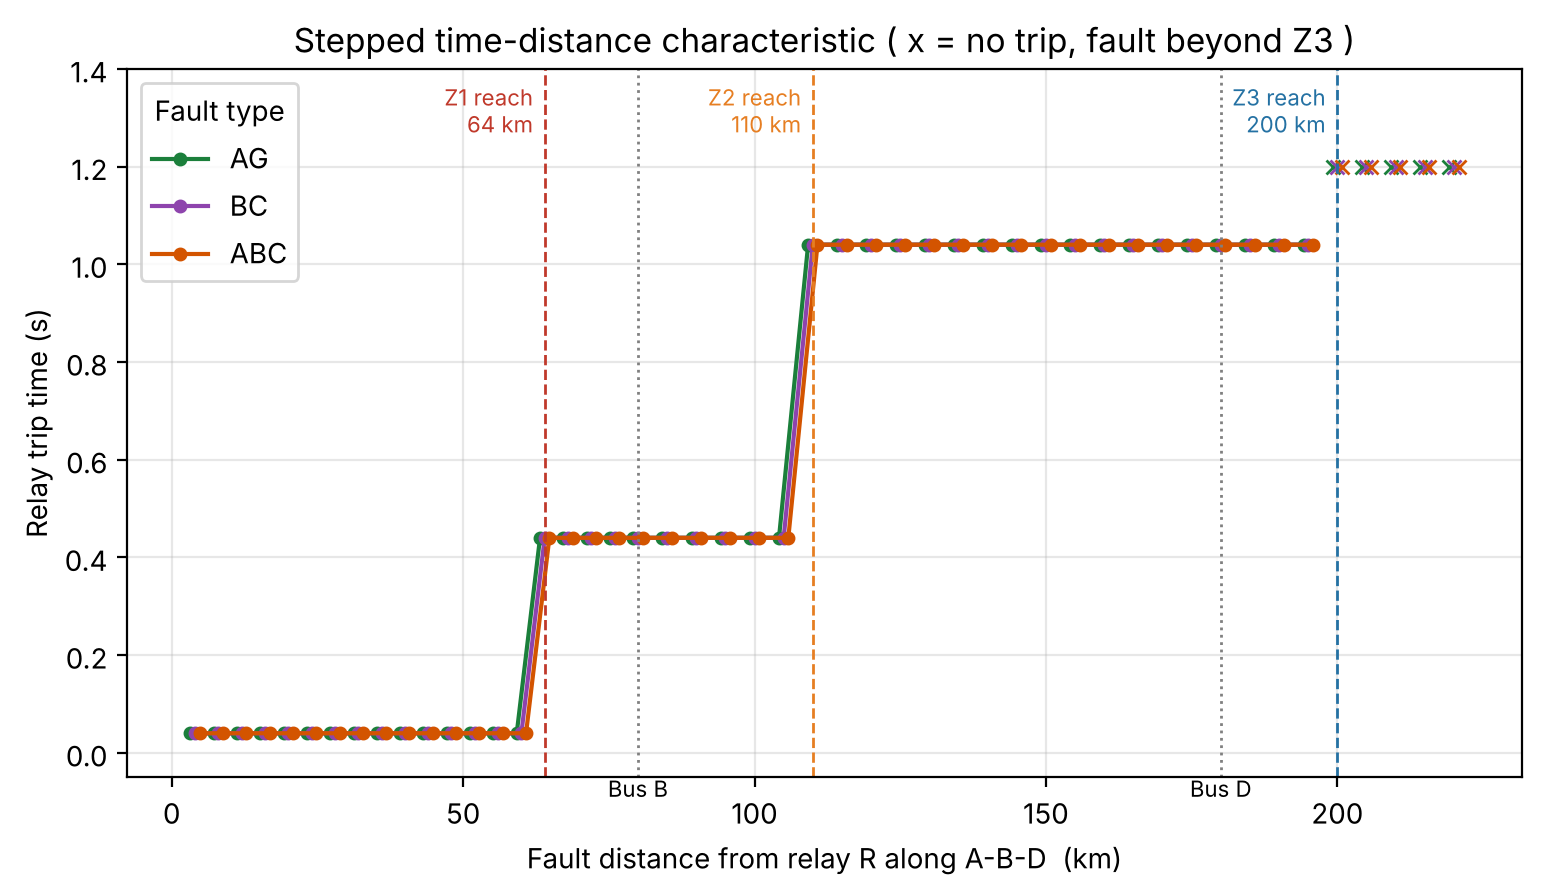
\includegraphics[width=0.9\textwidth]{figs/fig3_staircase.png}
\caption{Trip time versus fault distance along A-B-D. Crosses mark faults beyond Zone~3 (no trip).}\end{figure}
Of the 204 faults, 94.1\,\% picked up the ideal zone. All mismatches (4 per fault type) lie exactly on a reach boundary (64, 110 and 200\,km): fault resistance and noise move the apparent impedance just outside the circle, so the relay falls to the next slower zone (or does not operate at 200\,km); an example is the Line BC, 50\,\% row of Table~\ref{tab:sel}, which lies exactly at the Zone~2 reach of 110\,km.

\subsection{Effect of fault resistance}
\begin{figure}[H]\centering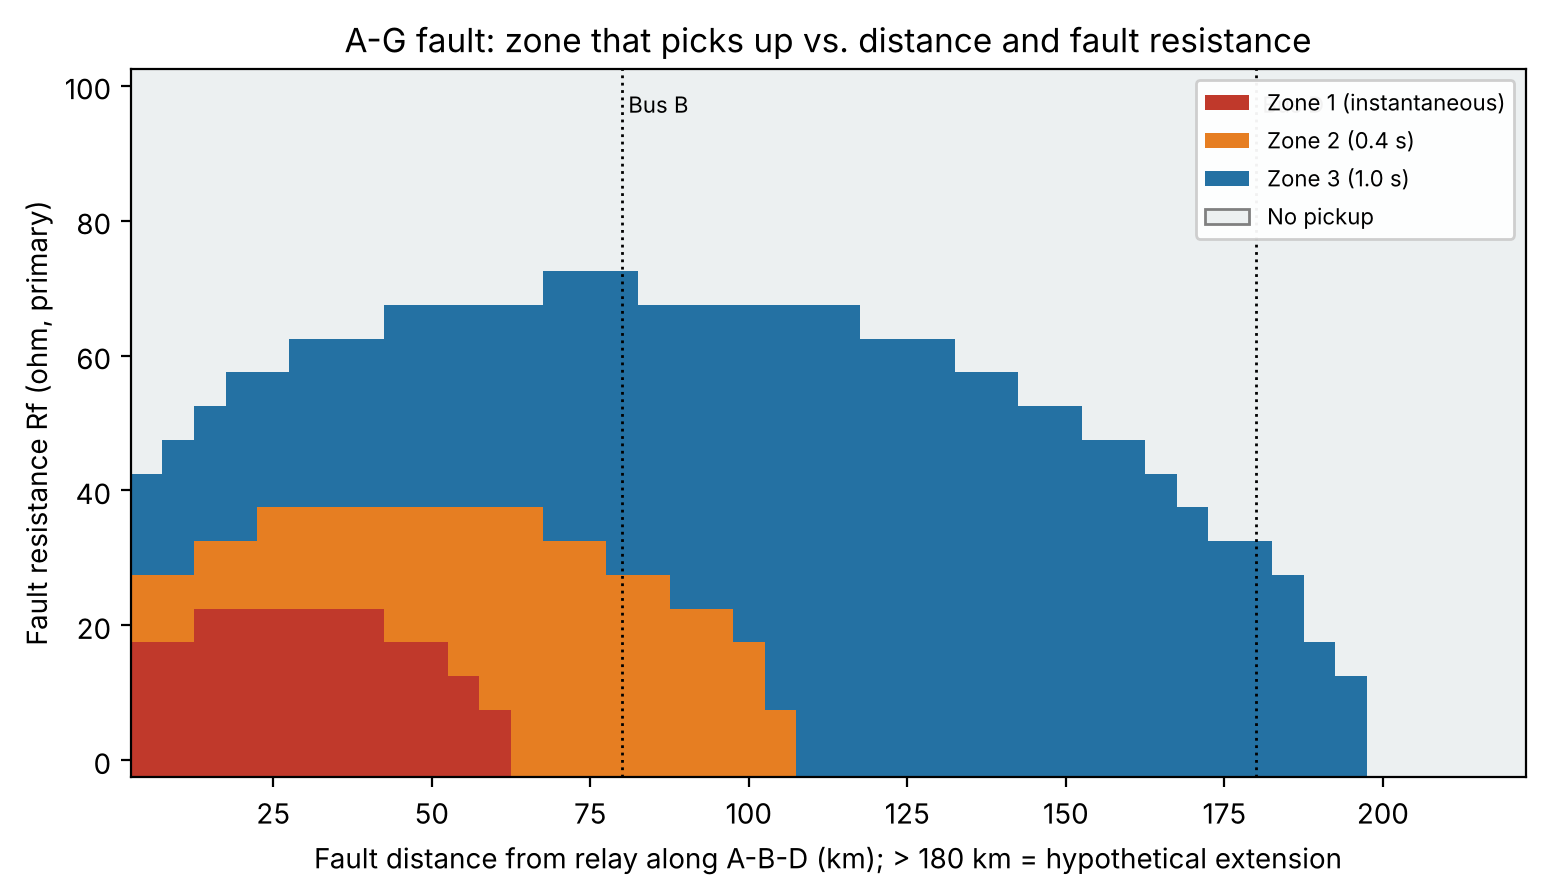
\includegraphics[width=0.9\textwidth]{figs/fig7_rf_map.png}
\caption{A-G faults: zone that picks up versus distance and fault resistance.}\end{figure}
The largest $R_f$ that still gives an instantaneous (Zone~1) trip is 20\,$\Omega$ at 16 and 32\,km and 15\,$\Omega$ at 48\,km; at the 64\,km reach limit no resistive fault is cleared instantly.

\section{Discussion}
\textbf{Agreement.} After DC-offset removal the impedance error is about 0.1\,\% on average (max 0.8\,\%), so the zone is correct everywhere except at the reach boundaries. Without the filter the error reaches 8\,\%, which is enough to move a fault near the Zone~1 boundary into Zone~2.\\
\textbf{Under-reach.} Fault resistance adds resistance to the apparent impedance and makes the fault look farther away. Remote infeed (not modelled) would add a further under-reach error. Zone~1 is set to 80\,\% so that errors do not make it overreach into the next line.\\
\textbf{Backup and coordination.} For a fault on BC or BD the local relay at Bus~B clears it with its own Zone~1, while relay R waits 0.4\,s (Zone~2) or 1.0\,s (Zone~3).\\
\textbf{Limitations.} Single source, no load, ideal CT/PT and ideal phase selection (only the faulted loop is evaluated); shunt capacitance and CT saturation are neglected. A practical relay would add load-encroachment and power-swing blocking.

\section{Conclusion}
A three-zone mho distance scheme was designed for line AB ($Z_1=26.11$, $Z_2=44.87$, $Z_3=81.58~\Omega$ primary; 0, 0.4 and 1.0\,s) and verified with 204 simulated faults of three types. With full-cycle DFT phasor estimation and DC-offset removal (mean error 0.1\,\%), the relay selected the correct zone away from the reach boundaries and produced the expected time staircase of 0.04, 0.44 and 1.04\,s. Fault resistance is the main practical cause of under-reach. The scheme coordinates with the downstream relays and does not operate for faults beyond Zone~3.

\section{GitHub Repository}
An interactive page (\texttt{docs/index.html}, hosted with GitHub Pages at \url{\DemoURL}) reproduces the sequence-network model in JavaScript. The user selects the fault type, distance and fault resistance and sees the apparent impedance on the R-X diagram with the zone and trip time. It shows the steady-state result, so it has no noise or DC offset. All code, results and this report are in \url{\RepoURL}.

\end{document}
